\begin{columns}[T]
	\begin{column}{0.02\textwidth}
	\end{column}
  \begin{column}{0.30\textwidth}
	  Stationary bulk convection \cite{chandrasekhar1981hydrodynamic}
	\hfill \break

  $Ra_{s} = \frac{3}{2} \left( 2 \pi^4 \right)^{\frac{1}{3}} {Ek}^{- \frac{4}{3}}$
  \end{column}
  \begin{column}{0.38\textwidth}
  Oscillatory convection (${Pr} > 0.68$) \cite{Horn2017}
  \hfill \break

  $Ra_{o} = \frac{3}{2} \left( 2 \pi \: {Pr} \right)^{\frac{4}{3}} \left(1 + {Pr} \right)^{- \frac{1}{3}} {Ek}^{-\frac{4}{3}}$
  \end{column}
  \begin{column}{0.30\textwidth}
  Wall-attached convection \cite{Herrmann1993}
  \hfill \break

  ${Ra_{w}} = \pi^{2} \left(6 \sqrt{3} \right)^{\frac{1}{2}} {Ek}^{-1}$
  \end{column}
\end{columns}
\hfill \break
\begin{columns}

	\begin{column}{0.02\textwidth}
	\end{column}
  \begin{column}{0.24\textwidth}
	\begin{tikzpicture}
		\node (COC1Prof) at (0,0) {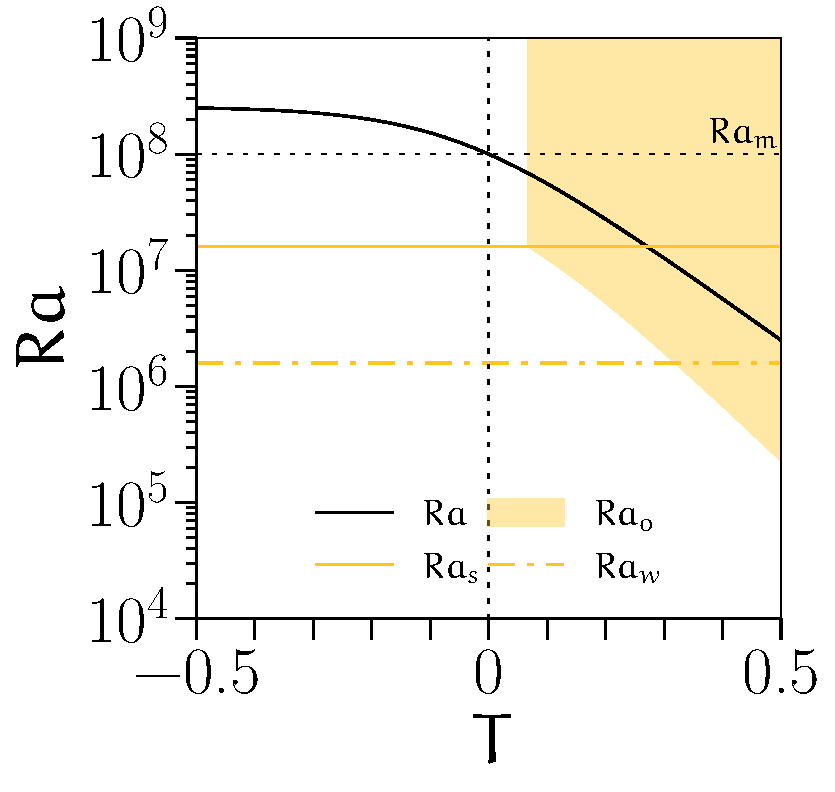
\includegraphics[width=\textwidth]{figs/ConvectionOnsetC1_1.pdf}};
		\node [rectangle, fill=none, align=center, text width=0.75\textwidth, xshift=0.075\textwidth, yshift=0.0\textwidth] (Title) at (COC1Prof.north) {\small $C1$, $Ro_m = 0.2$};
	\end{tikzpicture}
  \end{column}

  \begin{column}{0.24\textwidth}
	\begin{tikzpicture}
		\node (COC2Prof) at (0,0) {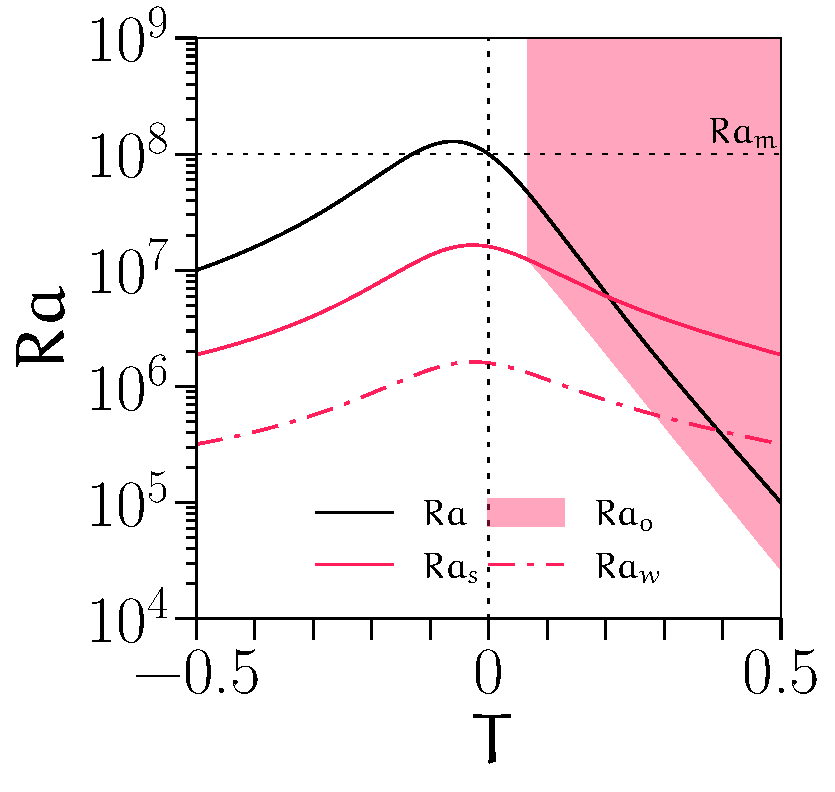
\includegraphics[width=\textwidth]{figs/ConvectionOnsetC1_2.pdf}};
		\node [rectangle, fill=none, align=center, text width=0.75\textwidth, xshift=0.075\textwidth, yshift=0.0\textwidth] (Title) at (COC2Prof.north) {\small $C2$ , $Ro_m = 0.2$};
	\end{tikzpicture}
  \end{column}

  \begin{column}{0.24\textwidth}
	\begin{tikzpicture}
		\node (COC3Prof) at (0,0) {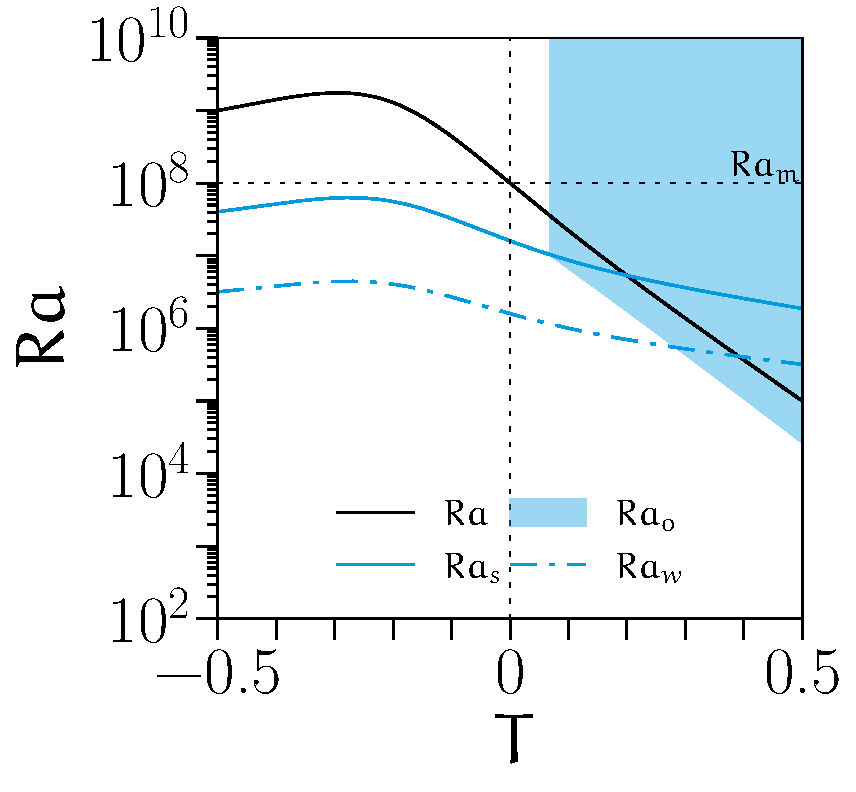
\includegraphics[width=\textwidth]{figs/ConvectionOnsetC1_3.pdf}};
		\node [rectangle, fill=none, align=center, text width=0.75\textwidth, xshift=0.075\textwidth, yshift=0.0\textwidth] (Title) at (COC3Prof.north) {\small $C3$ , $Ro_m = 0.2$};
	\end{tikzpicture}
	    %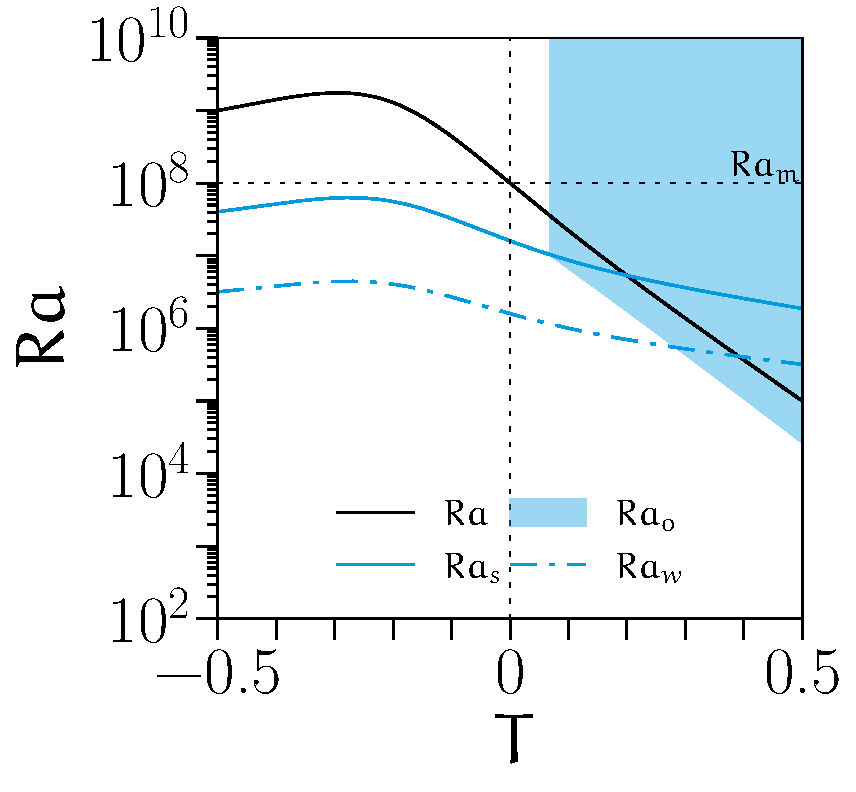
\includegraphics[width=\textwidth]{figs/ConvectionOnsetC1_3.pdf}
  \end{column}
  \begin{column}{0.24\textwidth}
	\begin{tikzpicture}
		\node (EkProf) at (0,0) {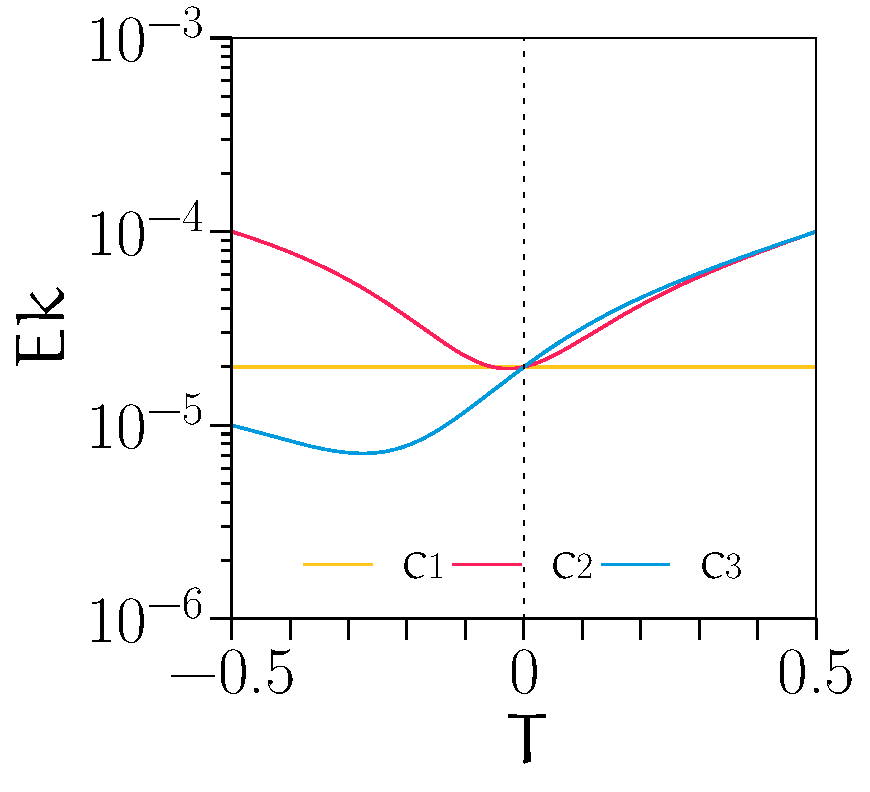
\includegraphics[width=\textwidth]{figs/Ek_Ra_C1.pdf}};
		\node [rectangle, fill=none, align=center, text width=0.75\textwidth, xshift=0.075\textwidth, yshift=0.0\textwidth] (Title) at (EkProf.north) {\small $Ek$ profile for $C1$};
	\end{tikzpicture}
      %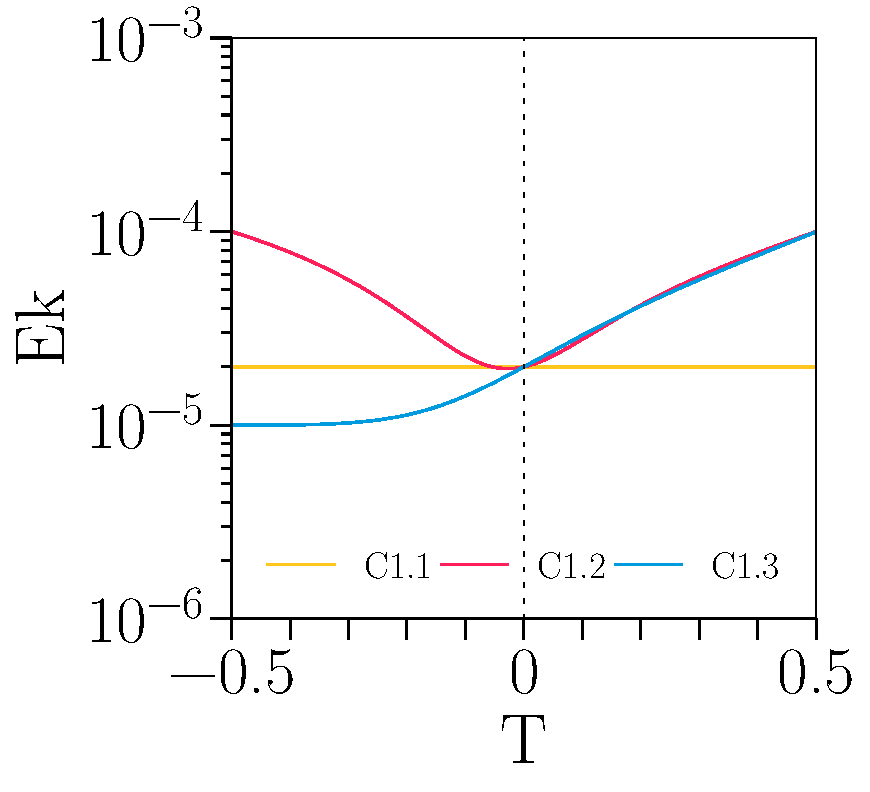
\includegraphics[width=\textwidth]{figs/Ek_Ra_C1_1.pdf}
  \end{column}
  \begin{column}{0.02\textwidth}
  \end{column}

\end{columns}
\begin{columns}

  \begin{column}{0.12\textwidth}
  \end{column}

  \begin{column}{0.24\textwidth}
	\begin{tikzpicture}
		\node (SCritC11Ro3) at (0,0) {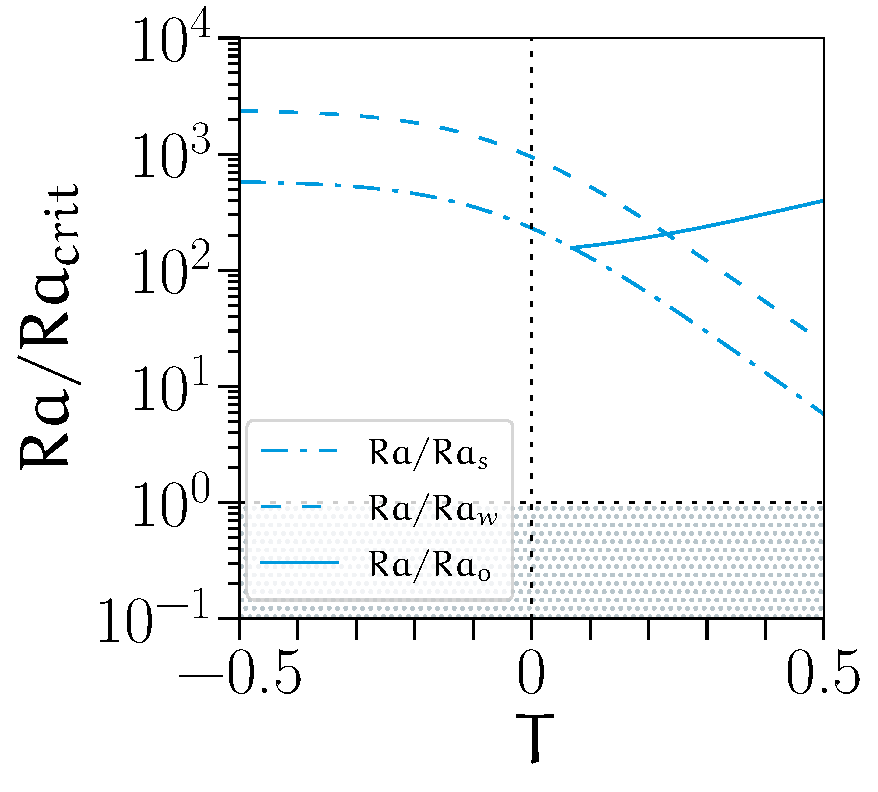
\includegraphics[width=\textwidth]{figs/SCritC11Ro3.pdf}};
		\node [rectangle, fill=none, align=center, text width=0.75\textwidth, xshift=0.075\textwidth, yshift=0.0\textwidth] (Title) at (SCritC11Ro3.north) {\small $C1$, $Ro_m=3.0$};
	\end{tikzpicture}
      %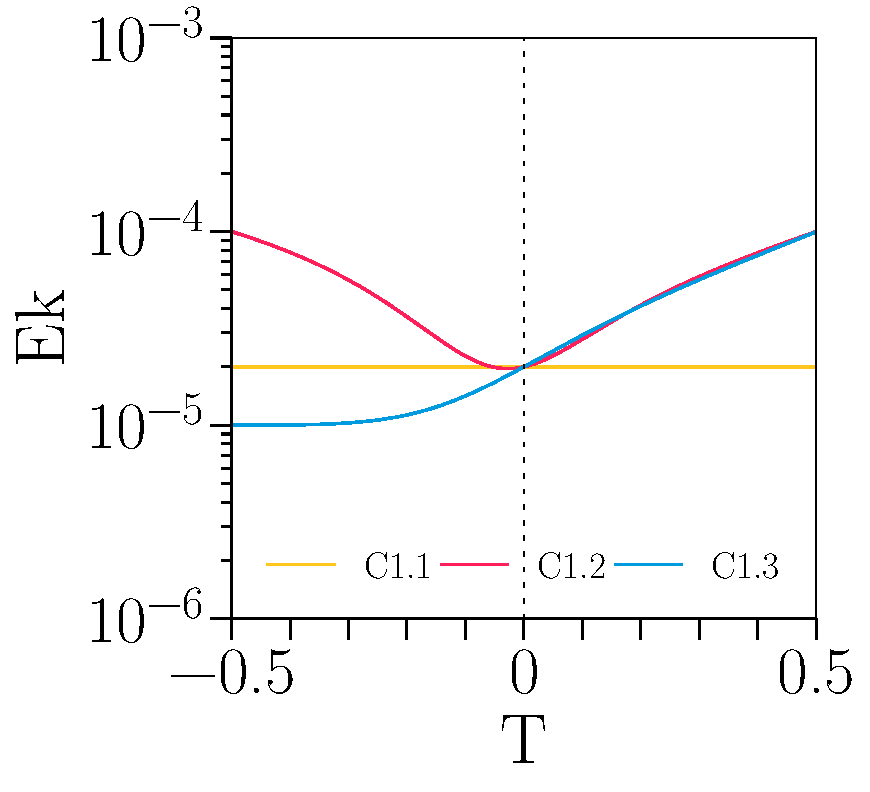
\includegraphics[width=\textwidth]{figs/Ek_Ra_C1_1.pdf}
  \end{column}
  \begin{column}{0.24\textwidth}
	\begin{tikzpicture}
		\node (SCritC11Ro1) at (0,0) {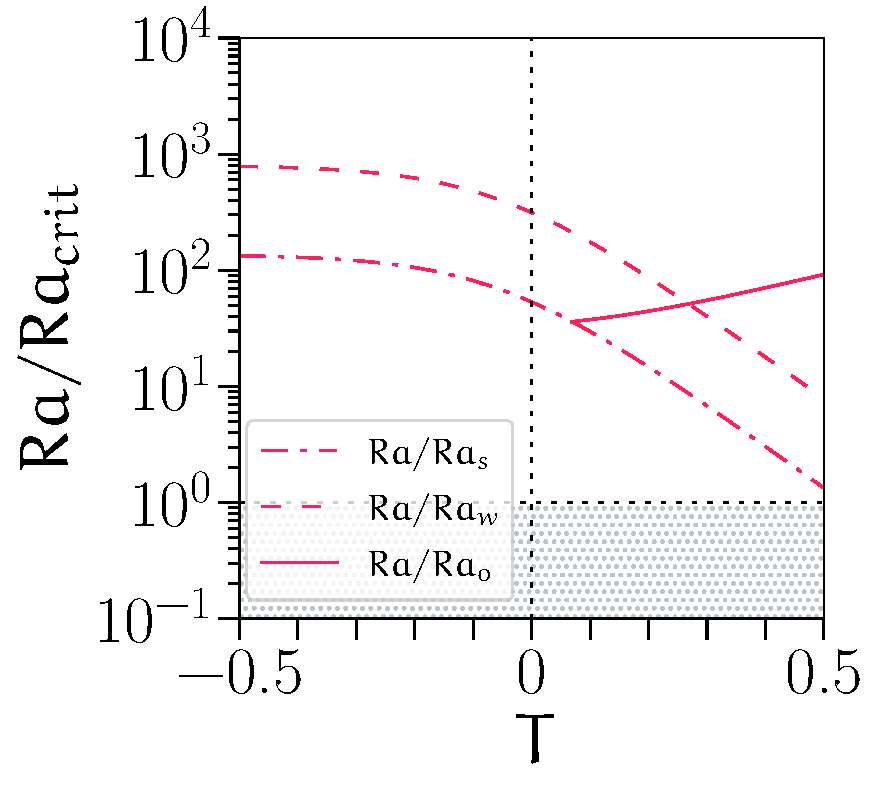
\includegraphics[width=\textwidth]{figs/SCritC11Ro1.pdf}};
		\node [rectangle, fill=none, align=center, text width=0.75\textwidth, xshift=0.075\textwidth, yshift=0.0\textwidth] (Title) at (SCritC11Ro1.north) {\small $C1$, $Ro_m=1.0$};
	\end{tikzpicture}
  \end{column}
  \begin{column}{0.24\textwidth}
	\begin{tikzpicture}
		\node (SCritC11Ro02) at (0,0) {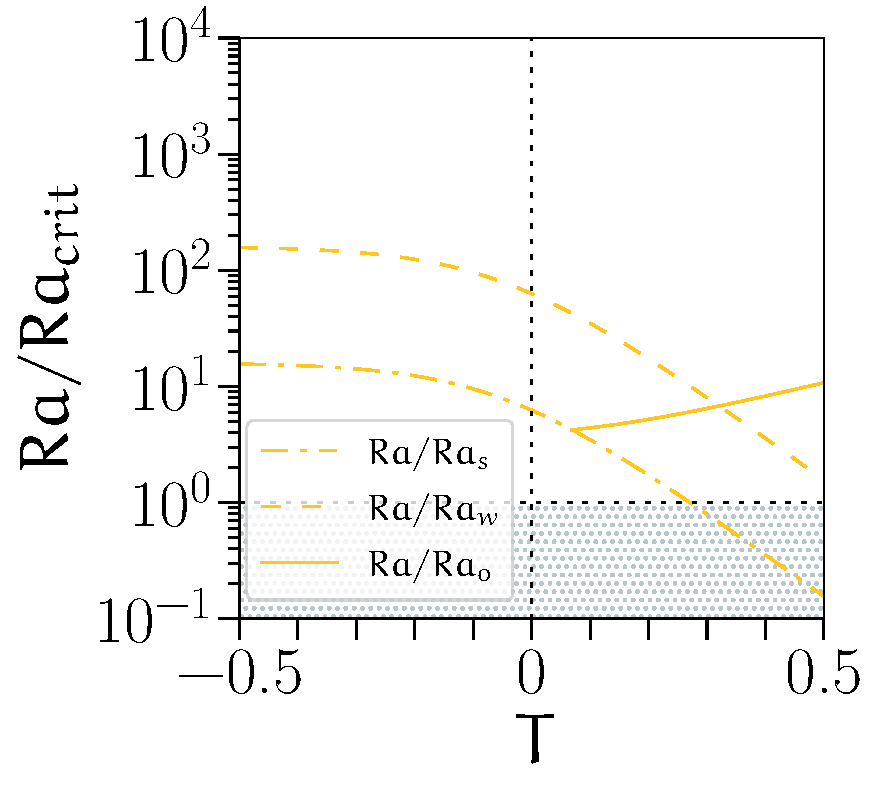
\includegraphics[width=\textwidth]{figs/SCritC11Ro02.pdf}};
		\node [rectangle, fill=none, align=center, text width=0.75\textwidth, xshift=0.075\textwidth, yshift=0.0\textwidth] (Title) at (SCritC11Ro02.north) {\small $C1$, $Ro_m=0.2$};
	\end{tikzpicture}
  \end{column}

  \begin{column}{0.12\textwidth}
  \end{column}
\end{columns}
